\documentclass[tikz,border=12pt]{standalone}
\usepackage[T1]{fontenc}
\usepackage{mathpazo}
\usepackage{amsmath,amssymb}
\usetikzlibrary{arrows.meta, positioning, calc}

\definecolor{stblue}{HTML}{7B97AD}
\definecolor{rwgold}{HTML}{B8995E}
\definecolor{sage}{HTML}{7A9A7E}
\definecolor{dkbrown}{HTML}{3D3530}
\definecolor{wmgray}{HTML}{7B7067}
\definecolor{cream}{HTML}{F9F6F0}
\definecolor{border}{HTML}{D4C9B8}
\definecolor{terracotta}{HTML}{C47A6A}
\definecolor{lavender}{HTML}{907EA0}

\begin{document}
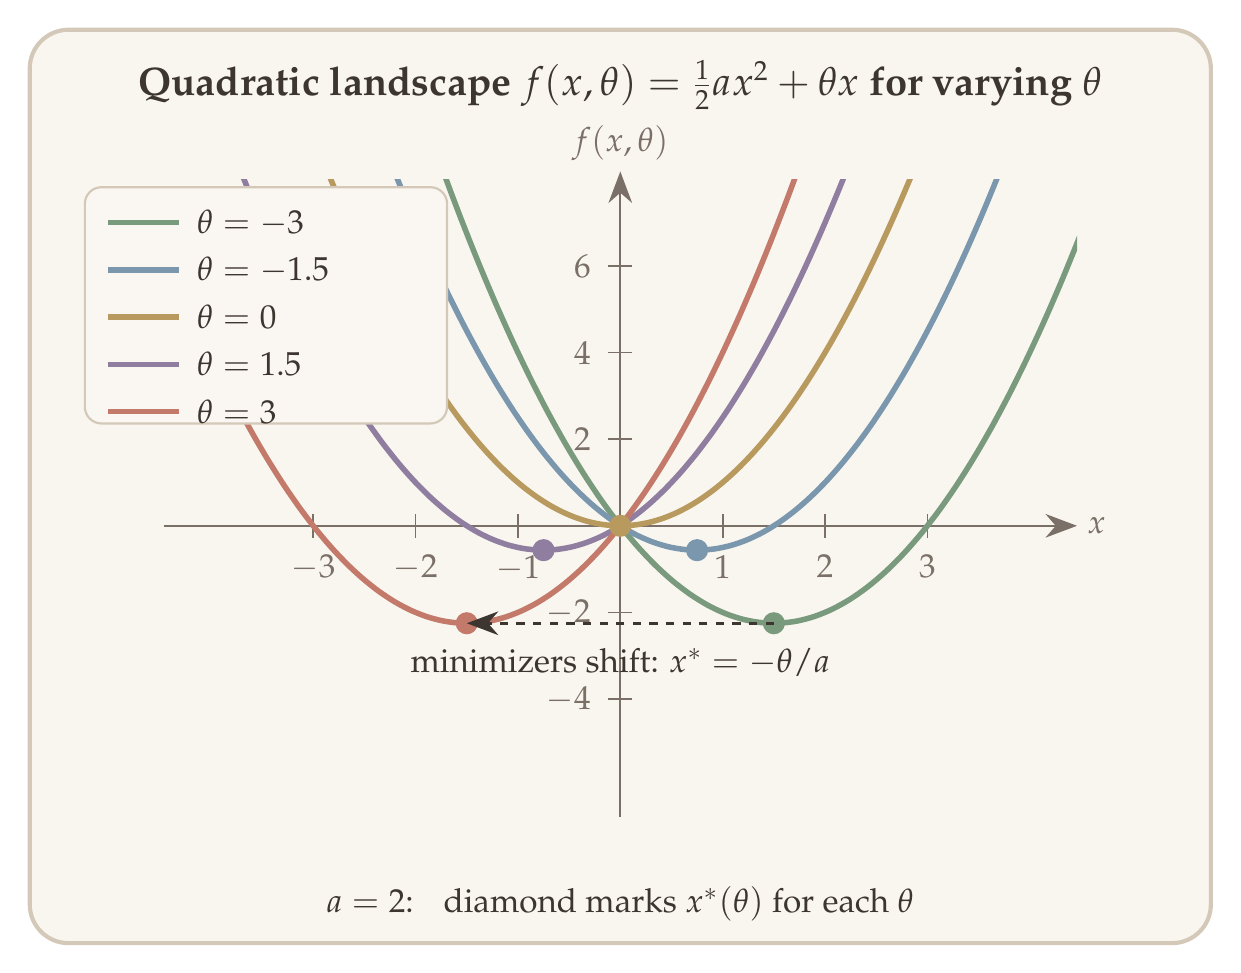
\begin{tikzpicture}[>={Stealth[length=4mm, width=3mm]}]

% Background
\fill[cream, rounded corners=14pt] (-0.5,-0.8) rectangle (14.5,10.8);
\draw[border, line width=1.5pt, rounded corners=14pt] (-0.5,-0.8) rectangle (14.5,10.8);

% Title
\node[text=dkbrown, font=\Large\bfseries] at (7,10.1)
  {Quadratic landscape $f(x,\theta) = \tfrac{1}{2}ax^2 + \theta x$ for varying $\theta$};

% Coordinate mapping:
% x-range: -4 to 4, center at canvas x=7
% y-range: -5 to 8, center at canvas y=4.5
% x-scale: 1.3, y-scale: 0.55

% Axes
\draw[wmgray, line width=0.8pt, ->] (1.2,4.5) -- (12.8,4.5)
  node[right, font=\large, text=wmgray] {$x$};
\draw[wmgray, line width=0.8pt, ->] (7.0,0.8) -- (7.0,9.0)
  node[above, font=\large, text=wmgray] {$f(x,\theta)$};

% x -> 7.0 + x*1.3
% y -> 4.5 + y*0.55

% Tick marks x-axis
\foreach \t/\lab in {-3/-3, -2/-2, -1/-1, 1/1, 2/2, 3/3} {
  \draw[wmgray, line width=0.6pt] ({7.0+\t*1.3},4.35) -- ({7.0+\t*1.3},4.65);
  \node[text=wmgray, font=\large, below] at ({7.0+\t*1.3},4.25) {$\lab$};
}

% Y-axis ticks
\foreach \v in {-4,-2,2,4,6} {
  \draw[wmgray, line width=0.6pt] (6.85,{4.5+\v*0.55}) -- (7.15,{4.5+\v*0.55});
  \node[text=wmgray, font=\large, left] at (6.75,{4.5+\v*0.55}) {\pgfmathprintnumber[fixed]{\v}};
}

% a = 2, f(x,theta) = x^2 + theta*x
% For each theta, plot parabola and mark minimizer x* = -theta/a = -theta/2
% Clip all curves to the plot area (axes range)

\begin{scope}
\clip (1.2,0.8) rectangle (12.8,8.9);

% theta = -3, x* = 1.5, f* = -2.25
\draw[sage, line width=2pt] plot[smooth, domain=-4:4.5, samples=50]
  ({7.0 + \x*1.3}, {4.5 + (\x*\x + (-3)*\x)*0.55});

% theta = -1.5, x* = 0.75, f* = -0.5625
\draw[stblue, line width=2pt] plot[smooth, domain=-3.5:4, samples=50]
  ({7.0 + \x*1.3}, {4.5 + (\x*\x + (-1.5)*\x)*0.55});

% theta = 0, x* = 0, f* = 0
\draw[rwgold, line width=2pt] plot[smooth, domain=-3:3, samples=50]
  ({7.0 + \x*1.3}, {4.5 + (\x*\x)*0.55});

% theta = 1.5, x* = -0.75, f* = -0.5625
\draw[lavender, line width=2pt] plot[smooth, domain=-4:3.5, samples=50]
  ({7.0 + \x*1.3}, {4.5 + (\x*\x + 1.5*\x)*0.55});

% theta = 3, x* = -1.5, f* = -2.25
\draw[terracotta, line width=2pt] plot[smooth, domain=-4.5:3, samples=50]
  ({7.0 + \x*1.3}, {4.5 + (\x*\x + 3*\x)*0.55});

\end{scope}

% Minimizer diamonds (drawn outside clip so they're always visible)
\fill[sage] ({7.0+1.5*1.3}, {4.5 + (1.5*1.5 + (-3)*1.5)*0.55})
  node[circle, inner sep=0pt, minimum size=8pt, fill=sage] {};
\fill[stblue] ({7.0+0.75*1.3}, {4.5 + (0.75*0.75 + (-1.5)*0.75)*0.55})
  node[circle, inner sep=0pt, minimum size=8pt, fill=stblue] {};
\fill[rwgold] (7.0, 4.5)
  node[circle, inner sep=0pt, minimum size=8pt, fill=rwgold] {};
\fill[lavender] ({7.0+(-0.75)*1.3}, {4.5 + (0.75*0.75 + 1.5*(-0.75))*0.55})
  node[circle, inner sep=0pt, minimum size=8pt, fill=lavender] {};
\fill[terracotta] ({7.0+(-1.5)*1.3}, {4.5 + (1.5*1.5 + 3*(-1.5))*0.55})
  node[circle, inner sep=0pt, minimum size=8pt, fill=terracotta] {};

% Legend
\fill[cream!90!white, rounded corners=6pt] (0.2,5.8) rectangle (4.8,8.8);
\draw[border, line width=0.8pt, rounded corners=6pt] (0.2,5.8) rectangle (4.8,8.8);

\draw[sage, line width=2pt] (0.5,8.35) -- (1.4,8.35);
\node[text=dkbrown, font=\large, right] at (1.5,8.35) {$\theta = -3$};
\draw[stblue, line width=2pt] (0.5,7.75) -- (1.4,7.75);
\node[text=dkbrown, font=\large, right] at (1.5,7.75) {$\theta = -1.5$};
\draw[rwgold, line width=2pt] (0.5,7.15) -- (1.4,7.15);
\node[text=dkbrown, font=\large, right] at (1.5,7.15) {$\theta = 0$};
\draw[lavender, line width=2pt] (0.5,6.55) -- (1.4,6.55);
\node[text=dkbrown, font=\large, right] at (1.5,6.55) {$\theta = 1.5$};
\draw[terracotta, line width=2pt] (0.5,5.95) -- (1.4,5.95);
\node[text=dkbrown, font=\large, right] at (1.5,5.95) {$\theta = 3$};

% Annotation: path of minimizers
\draw[dkbrown, line width=1pt, dashed, ->]
  ({7.0+1.5*1.3}, {4.5-2.25*0.55}) -- ({7.0+(-1.5)*1.3}, {4.5-2.25*0.55});
\node[text=dkbrown, font=\large] at (7.0, {4.5-2.25*0.55-0.5})
  {minimizers shift: $x^* = -\theta/a$};

% Bottom note
\node[text=dkbrown, font=\large] at (7,-0.3)
  {$a = 2$: \; diamond marks $x^*(\theta)$ for each $\theta$};

\end{tikzpicture}
\end{document}
